% Options for packages loaded elsewhere
\PassOptionsToPackage{unicode}{hyperref}
\PassOptionsToPackage{hyphens}{url}
\PassOptionsToPackage{dvipsnames,svgnames,x11names}{xcolor}
%
\documentclass[
  letterpaper,
  DIV=11,
  numbers=noendperiod]{scrartcl}

\usepackage{amsmath,amssymb}
\usepackage{iftex}
\ifPDFTeX
  \usepackage[T1]{fontenc}
  \usepackage[utf8]{inputenc}
  \usepackage{textcomp} % provide euro and other symbols
\else % if luatex or xetex
  \usepackage{unicode-math}
  \defaultfontfeatures{Scale=MatchLowercase}
  \defaultfontfeatures[\rmfamily]{Ligatures=TeX,Scale=1}
\fi
\usepackage{lmodern}
\ifPDFTeX\else  
    % xetex/luatex font selection
\fi
% Use upquote if available, for straight quotes in verbatim environments
\IfFileExists{upquote.sty}{\usepackage{upquote}}{}
\IfFileExists{microtype.sty}{% use microtype if available
  \usepackage[]{microtype}
  \UseMicrotypeSet[protrusion]{basicmath} % disable protrusion for tt fonts
}{}
\makeatletter
\@ifundefined{KOMAClassName}{% if non-KOMA class
  \IfFileExists{parskip.sty}{%
    \usepackage{parskip}
  }{% else
    \setlength{\parindent}{0pt}
    \setlength{\parskip}{6pt plus 2pt minus 1pt}}
}{% if KOMA class
  \KOMAoptions{parskip=half}}
\makeatother
\usepackage{xcolor}
\setlength{\emergencystretch}{3em} % prevent overfull lines
\setcounter{secnumdepth}{-\maxdimen} % remove section numbering
% Make \paragraph and \subparagraph free-standing
\makeatletter
\ifx\paragraph\undefined\else
  \let\oldparagraph\paragraph
  \renewcommand{\paragraph}{
    \@ifstar
      \xxxParagraphStar
      \xxxParagraphNoStar
  }
  \newcommand{\xxxParagraphStar}[1]{\oldparagraph*{#1}\mbox{}}
  \newcommand{\xxxParagraphNoStar}[1]{\oldparagraph{#1}\mbox{}}
\fi
\ifx\subparagraph\undefined\else
  \let\oldsubparagraph\subparagraph
  \renewcommand{\subparagraph}{
    \@ifstar
      \xxxSubParagraphStar
      \xxxSubParagraphNoStar
  }
  \newcommand{\xxxSubParagraphStar}[1]{\oldsubparagraph*{#1}\mbox{}}
  \newcommand{\xxxSubParagraphNoStar}[1]{\oldsubparagraph{#1}\mbox{}}
\fi
\makeatother


\providecommand{\tightlist}{%
  \setlength{\itemsep}{0pt}\setlength{\parskip}{0pt}}\usepackage{longtable,booktabs,array}
\usepackage{calc} % for calculating minipage widths
% Correct order of tables after \paragraph or \subparagraph
\usepackage{etoolbox}
\makeatletter
\patchcmd\longtable{\par}{\if@noskipsec\mbox{}\fi\par}{}{}
\makeatother
% Allow footnotes in longtable head/foot
\IfFileExists{footnotehyper.sty}{\usepackage{footnotehyper}}{\usepackage{footnote}}
\makesavenoteenv{longtable}
\usepackage{graphicx}
\makeatletter
\newsavebox\pandoc@box
\newcommand*\pandocbounded[1]{% scales image to fit in text height/width
  \sbox\pandoc@box{#1}%
  \Gscale@div\@tempa{\textheight}{\dimexpr\ht\pandoc@box+\dp\pandoc@box\relax}%
  \Gscale@div\@tempb{\linewidth}{\wd\pandoc@box}%
  \ifdim\@tempb\p@<\@tempa\p@\let\@tempa\@tempb\fi% select the smaller of both
  \ifdim\@tempa\p@<\p@\scalebox{\@tempa}{\usebox\pandoc@box}%
  \else\usebox{\pandoc@box}%
  \fi%
}
% Set default figure placement to htbp
\def\fps@figure{htbp}
\makeatother

\KOMAoption{captions}{tableheading}
\makeatletter
\@ifpackageloaded{caption}{}{\usepackage{caption}}
\AtBeginDocument{%
\ifdefined\contentsname
  \renewcommand*\contentsname{Table of contents}
\else
  \newcommand\contentsname{Table of contents}
\fi
\ifdefined\listfigurename
  \renewcommand*\listfigurename{List of Figures}
\else
  \newcommand\listfigurename{List of Figures}
\fi
\ifdefined\listtablename
  \renewcommand*\listtablename{List of Tables}
\else
  \newcommand\listtablename{List of Tables}
\fi
\ifdefined\figurename
  \renewcommand*\figurename{Figure}
\else
  \newcommand\figurename{Figure}
\fi
\ifdefined\tablename
  \renewcommand*\tablename{Table}
\else
  \newcommand\tablename{Table}
\fi
}
\@ifpackageloaded{float}{}{\usepackage{float}}
\floatstyle{ruled}
\@ifundefined{c@chapter}{\newfloat{codelisting}{h}{lop}}{\newfloat{codelisting}{h}{lop}[chapter]}
\floatname{codelisting}{Listing}
\newcommand*\listoflistings{\listof{codelisting}{List of Listings}}
\makeatother
\makeatletter
\makeatother
\makeatletter
\@ifpackageloaded{caption}{}{\usepackage{caption}}
\@ifpackageloaded{subcaption}{}{\usepackage{subcaption}}
\makeatother

\usepackage{bookmark}

\IfFileExists{xurl.sty}{\usepackage{xurl}}{} % add URL line breaks if available
\urlstyle{same} % disable monospaced font for URLs
\hypersetup{
  pdftitle={MicrogliaTRAP},
  colorlinks=true,
  linkcolor={blue},
  filecolor={Maroon},
  citecolor={Blue},
  urlcolor={Blue},
  pdfcreator={LaTeX via pandoc}}


\title{MicrogliaTRAP}
\author{Evgenii O. Tretiakov, PhD}
\date{}

\begin{document}
\maketitle


\subsection{TREM2 Expression Analysis Across Hypothalamic
Regions}\label{trem2-expression-analysis-across-hypothalamic-regions}

\subsubsection{Methods}\label{methods}

TREM2 expression was analyzed across different hypothalamic regions
using single-nucleus RNA sequencing data. Following quality control and
normalization, we performed integrated analysis of multiple datasets
(Figure~\ref{fig-integrated-analysis}).

\begin{figure}[H]

\centering{

\pandocbounded{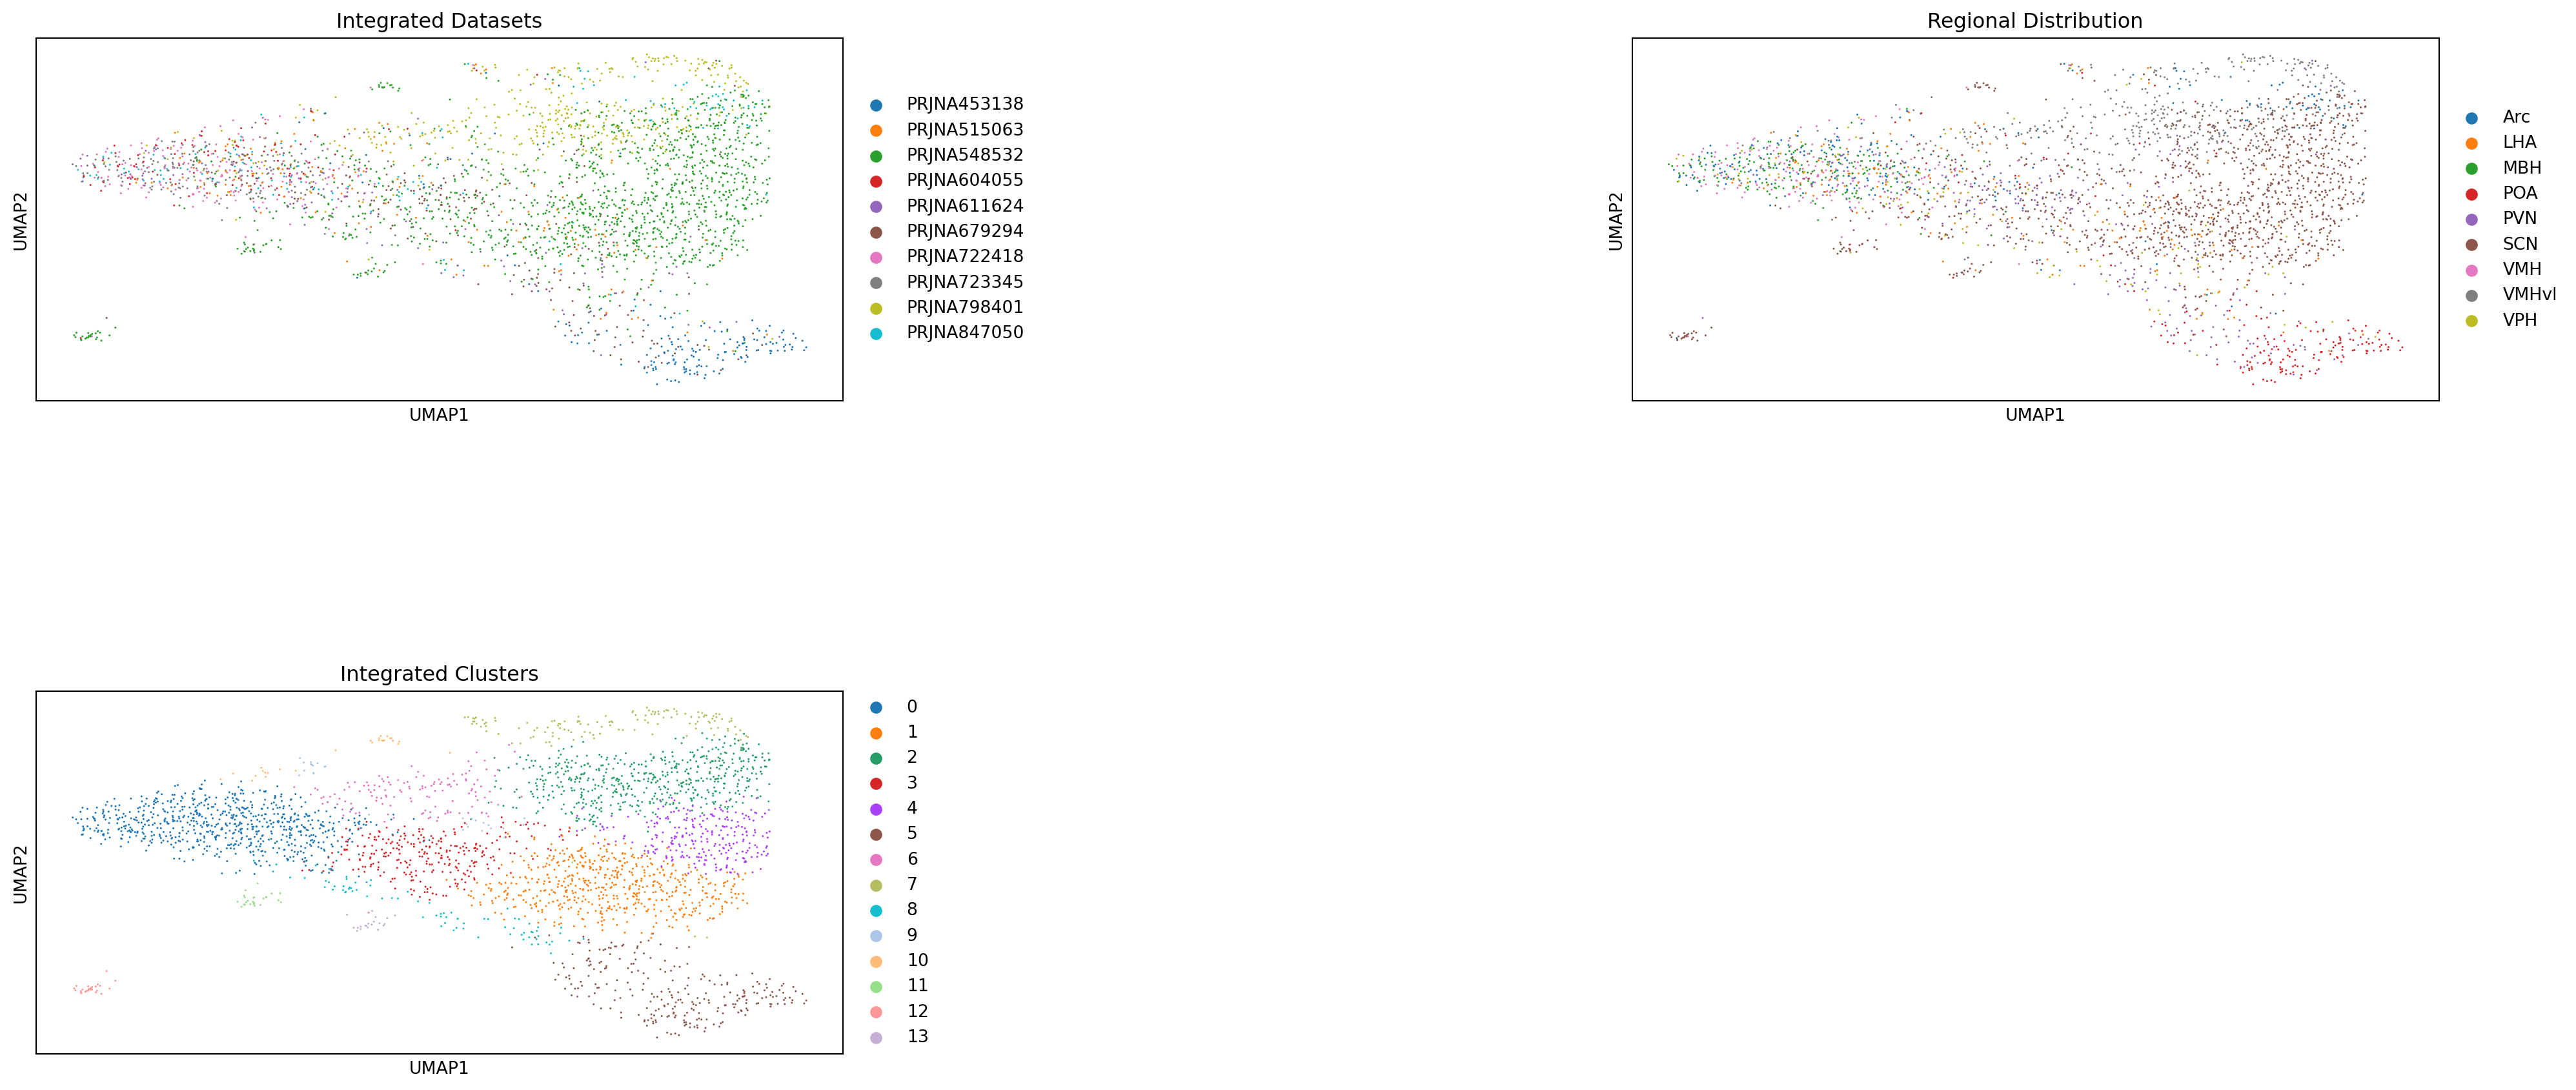
\includegraphics[keepaspectratio]{index_files/figure-latex/notebooks-eda-fig-integrated-analysis-output-1.png}}

}

\caption{\label{fig-integrated-analysis}Analysis of batch-corrected
microglial data. (A) UMAP visualization after integration shows reduced
batch effects. (B) Refined clustering based on integrated data reveals
distinct microglial subpopulations. (C) Distribution of cells by
hypothalamic region demonstrates regional heterogeneity of microglia.}

\end{figure}%

\textsubscript{Source:
\href{https://EugOT.github.io/MicrogliaTRAP/notebooks/eda-preview.html\#cell-fig-integrated-analysis}{Comprehensive
analysis of hypothalamic microglia across multiple}}

Initial clustering revealed distinct microglial populations across
hypothalamic regions, further refined through batch correction and
integration of 20 independent datasets.

\textbf{Dataset Summary:}\\
The combined dataset comprised \textbf{271,739 cells} drawn from
\textbf{12 independent datasets} (for now; we have 20 in total). After
exclusion of sex-specific genes (using the list provided below) and
applying a super conservative filtering strategy, \textbf{3,108
high-confidence microglia} were retained for downstream analysis.

\textbf{Filtering Details and Gene Lists:}\\
To ensure the highest specificity in microglia selection, we computed a
composite positivity score for each cell. This score integrates:

\begin{itemize}
\tightlist
\item
  \textbf{Expression of Primary (Highly Specific) Markers:}\\
  These genes must be robustly expressed:

  \begin{itemize}
  \tightlist
  \item
    \emph{Primary Markers:}\\
    \texttt{P2ry12,\ Tmem119,\ Siglech,\ Fcrls,\ Gpr34,\ Hexb}
  \end{itemize}
\item
  \textbf{Expression of Secondary (Supportive) Markers:}\\
  These genes serve as supplemental evidence of microglial identity:

  \begin{itemize}
  \tightlist
  \item
    \emph{Secondary Markers:}\\
    \texttt{Trem2,\ Aif1,\ Sall1}
  \end{itemize}
\item
  \textbf{Absence of Negative (Exclusion) Markers:}\\
  Any detectable expression of these genes indicates contamination from
  other cell types, so such cells are excluded:

  \begin{itemize}
  \tightlist
  \item
    \emph{Negative Markers:}\\
    \texttt{Snap25,\ Rbfox3,\ Dlx5,\ Elavl4,\ Stmn2,\ Th,\ Slc17a6,\ Gad1,\ Gad2,\ Npy,\ Agrp,\ Crh,\ Trh,\ Avp,\ Pomc,\ Hcrt,\ Oxt,\ Vim,\ Nes,\ Enkur,\ Foxj1,\ Kif6,\ Kif9,\ Hydin,\ Mog,\ Mbp,\ Plp1,\ Cnp,\ Mag,\ Opalin,\ Sox10,\ Olig1,\ Olig2,\ Pdgfra,\ Pdgfrb,\ Gpr17,\ Ugt8a,\ Sema3c,\ Sema4d,\ Sema4f,\ Gpr37,\ Cspg4,\ Lingo1,\ Rgs5,\ Des,\ Acta2,\ Pecam1,\ Cldn5,\ Cd248,\ Myh11,\ Cdh5,\ Fgf10,\ Rax,\ Gfap,\ Aldh1l1,\ Aqp4,\ Agt,\ Gja1,\ Hepacam,\ Htra1,\ Ndrg2,\ Ntsr2,\ Ntrk2,\ Slc1a3,\ Slc6a11,\ Slc1a2,\ Apoe,\ Adcyap1r1}
  \end{itemize}
\item
  \textbf{Exclusion of Sex-Specific Genes:}\\
  These genes are filtered out to remove sex-related differences:

  \begin{itemize}
  \tightlist
  \item
    \emph{Sex-Specific Genes:}\\
    \texttt{Ehd2,\ Espl1,\ Jarid1d,\ Pnpla4,\ Rps4y1,\ Xist,\ Tsix,\ Eif2s3y,\ Ddx3y,\ Uty,\ Kdm5d}
  \end{itemize}
\end{itemize}

In this super conservative filtering, only cells with a composite score
exceeding a defined threshold---and exhibiting no detectable expression
of any negative markers---were selected as microglia. This approach may
be further adapted (i.e.~by relaxing or tightening thresholds) depending
on future experimental needs.

\subsubsection{Results}\label{results}

\paragraph{Regional Expression
Patterns}\label{regional-expression-patterns}

Analysis of TREM2 expression revealed significant heterogeneity across
hypothalamic regions (F = 302.35, p = 2.58e-4).
Figure~\ref{fig-trem2-region} shows the distribution of TREM2 expression
across different regions.

\begin{figure}[H]

\centering{

\pandocbounded{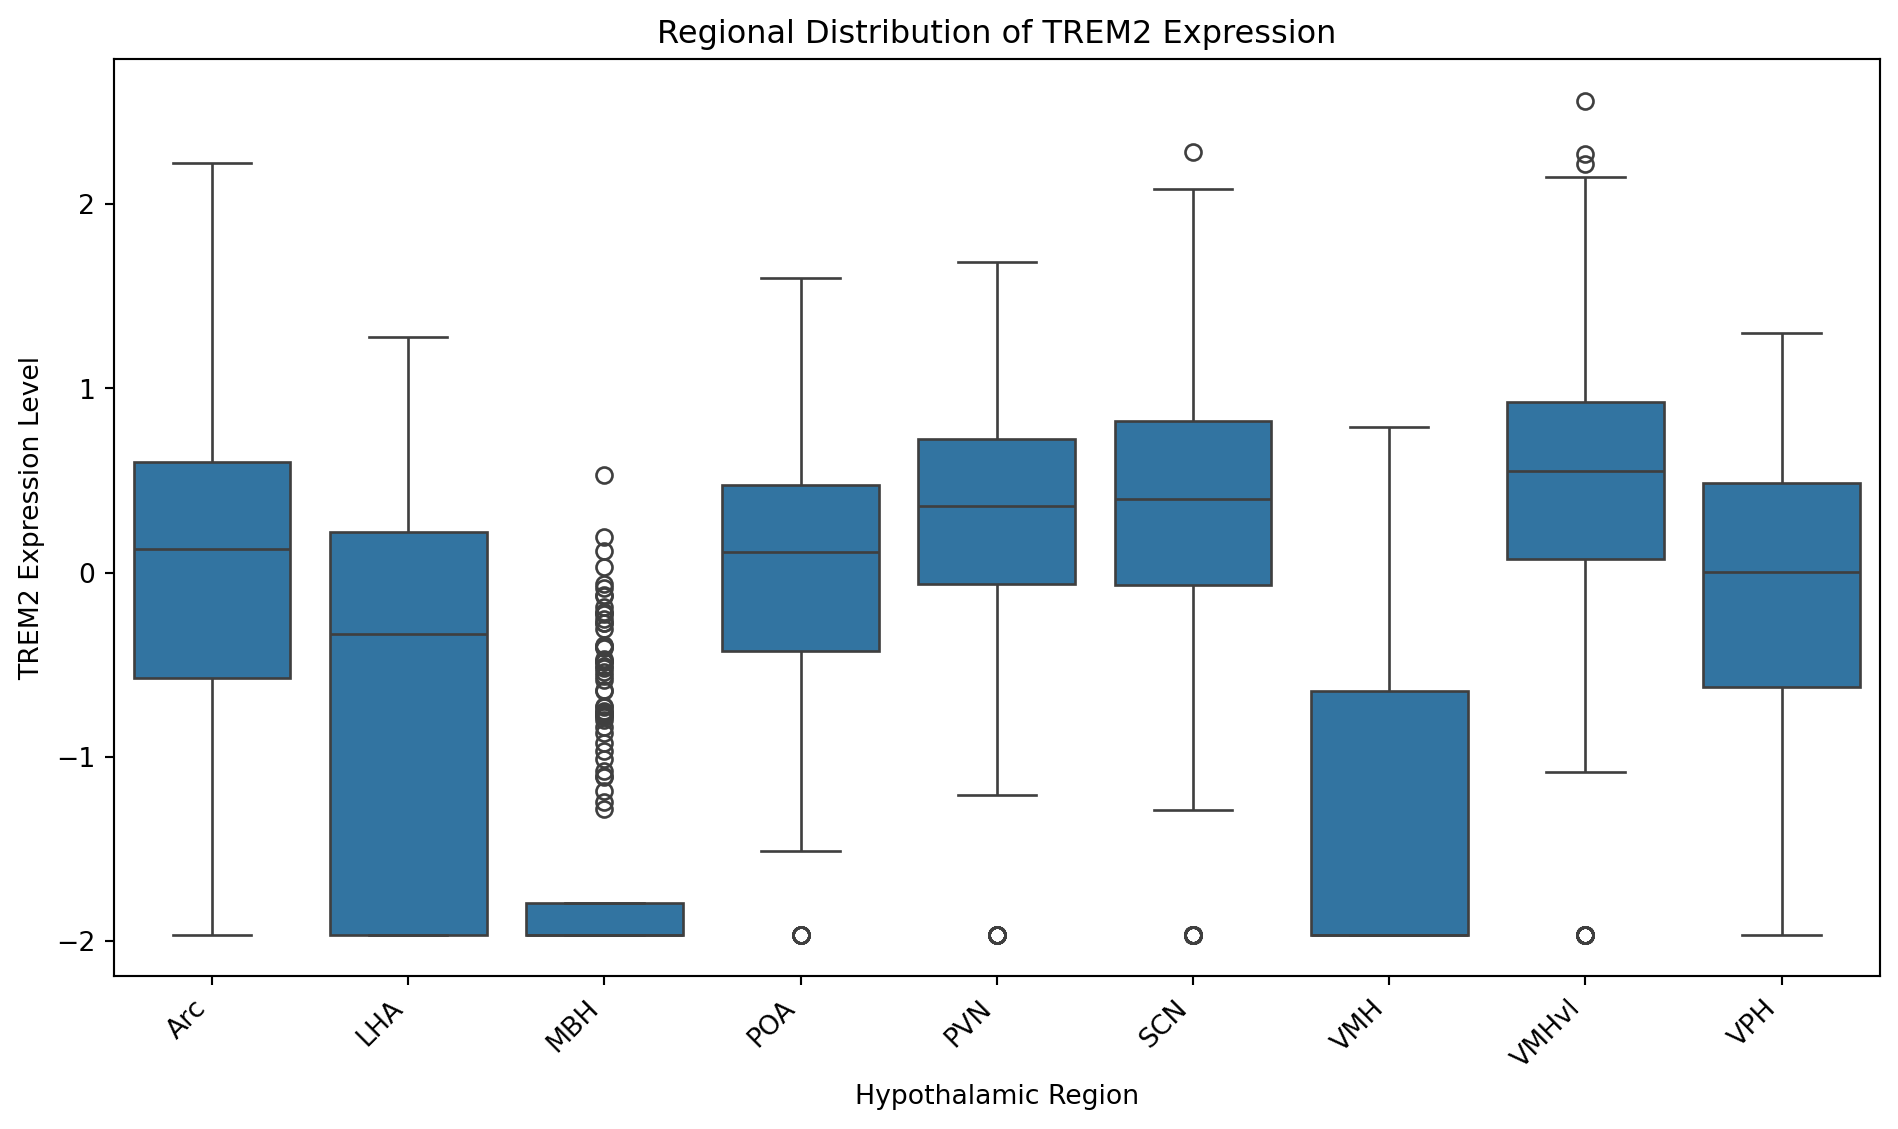
\includegraphics[keepaspectratio]{index_files/figure-latex/notebooks-eda-fig-trem2-region-output-1.png}}

}

\caption{\label{fig-trem2-region}TREM2 expression levels across
different hypothalamic regions. Box plots show the median, quartiles,
and distribution of TREM2 expression in each anatomically distinct
region. Whiskers extend to 1.5 times the interquartile range.}

\end{figure}%

\textsubscript{Source:
\href{https://EugOT.github.io/MicrogliaTRAP/notebooks/eda-preview.html\#cell-fig-trem2-region}{Comprehensive
analysis of hypothalamic microglia across multiple}}

The highest TREM2 expression was observed in the SCN (mean = 0.436 ±
0.689), followed by the PVN (0.296 ± 0.799). In contrast, the MBH showed
the lowest expression (-1.376 ± 0.604), followed by the MnPO (-1.241 ±
0.057).

\paragraph{Cluster-Specific
Expression}\label{cluster-specific-expression}

TREM2 expression varied significantly across microglial clusters
(Figure~\ref{fig-trem2-clusters}), suggesting functional heterogeneity
within the microglial population.

\begin{figure}[H]

\centering{

\pandocbounded{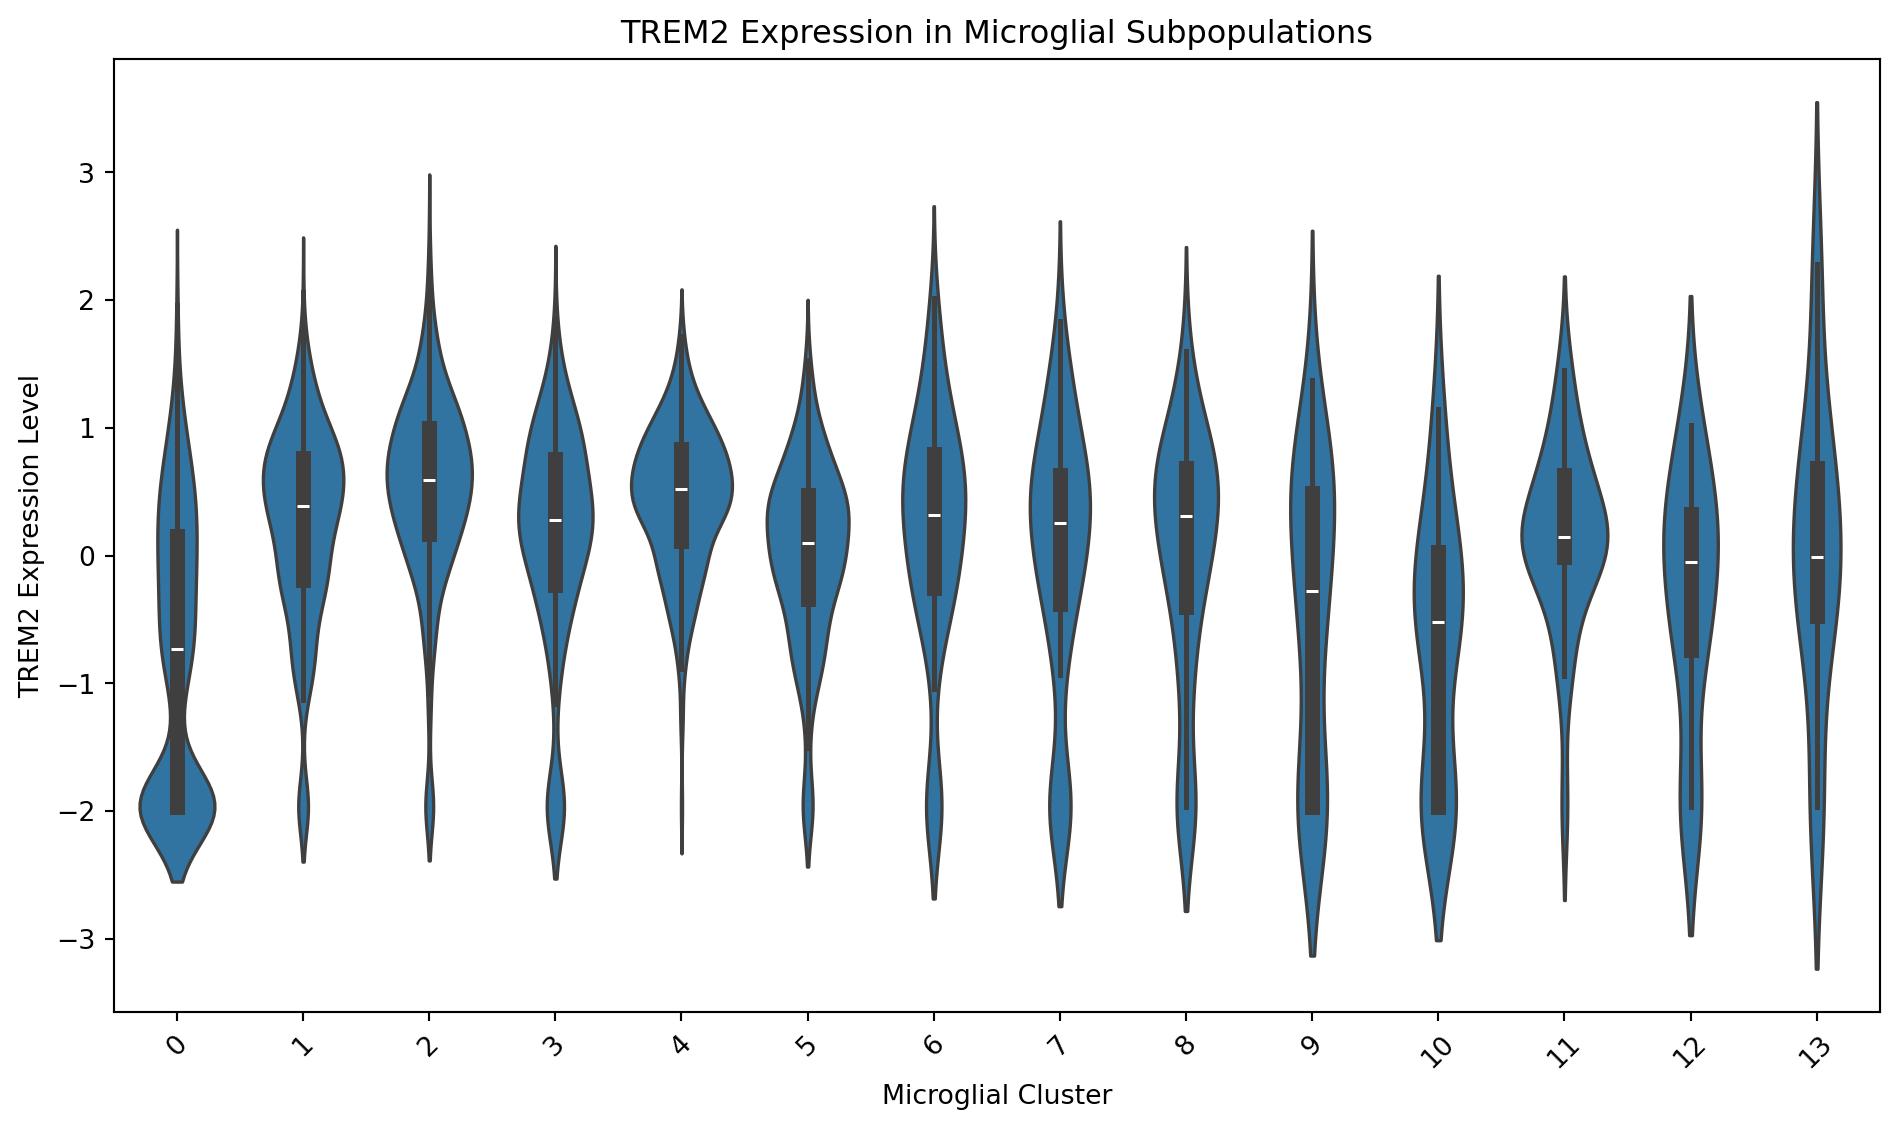
\includegraphics[keepaspectratio]{index_files/figure-latex/notebooks-eda-fig-trem2-clusters-output-1.png}}

}

\caption{\label{fig-trem2-clusters}Distribution of TREM2 expression
across identified microglial clusters. Violin plots demonstrate the full
distribution of expression levels within each cluster, with embedded box
plots showing median and quartile values.}

\end{figure}%

\textsubscript{Source:
\href{https://EugOT.github.io/MicrogliaTRAP/notebooks/eda-preview.html\#cell-fig-trem2-clusters}{Comprehensive
analysis of hypothalamic microglia across multiple}}

\paragraph{Spatial Distribution}\label{spatial-distribution}

UMAP visualization of TREM2 expression (Figure~\ref{fig-trem2-umap})
revealed distinct spatial patterns, indicating regional specialization
of TREM2-expressing microglia.

\begin{figure}[H]

\centering{

\pandocbounded{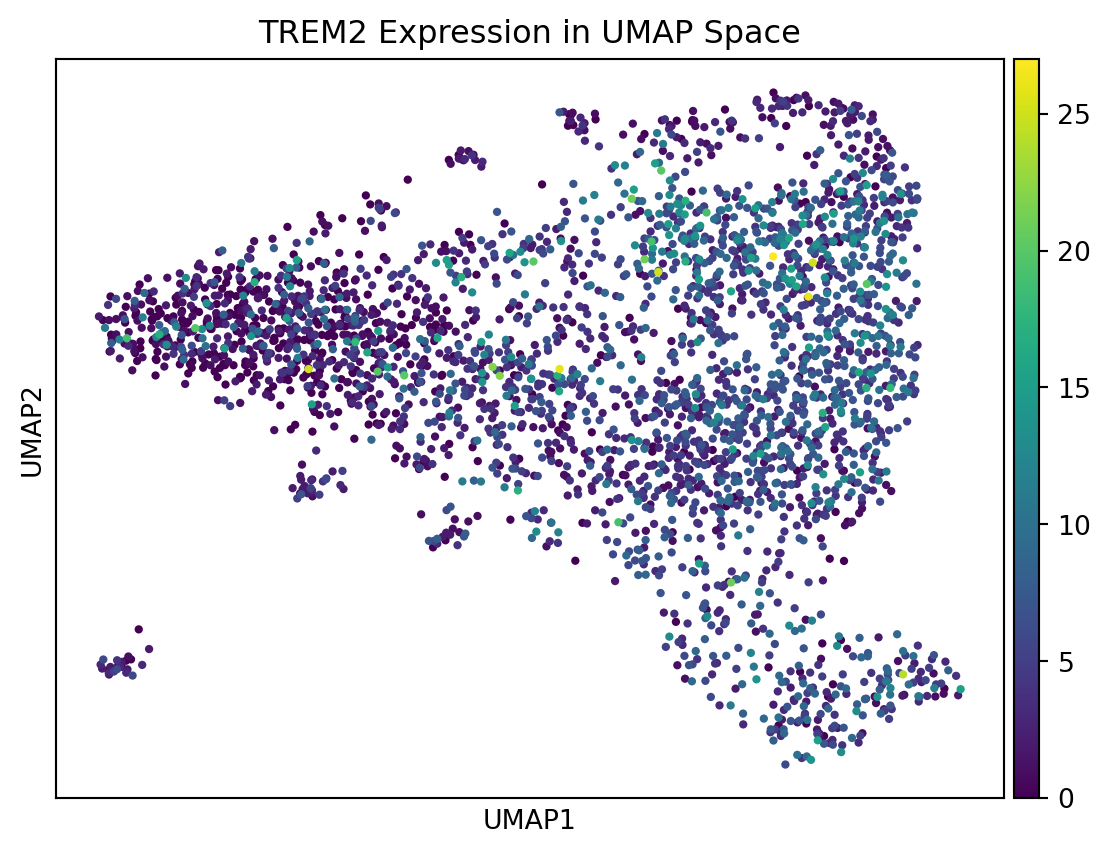
\includegraphics[keepaspectratio]{index_files/figure-latex/notebooks-eda-fig-trem2-umap-output-1.png}}

}

\caption{\label{fig-trem2-umap}UMAP visualization of TREM2 expression
across all microglia. Color intensity represents TREM2 expression level,
showing the spatial distribution of TREM2-expressing cells in the
UMAP-reduced 2-dimensional space.}

\end{figure}%

\textsubscript{Source:
\href{https://EugOT.github.io/MicrogliaTRAP/notebooks/eda-preview.html\#cell-fig-trem2-umap}{Comprehensive
analysis of hypothalamic microglia across multiple}}

\paragraph{Gene Co-expression
Analysis}\label{gene-co-expression-analysis}

To understand the regulatory network associated with TREM2, we analyzed
its correlation with other microglial markers
(Figure~\ref{fig-trem2-correlations}).

\begin{figure}[H]

\centering{

\pandocbounded{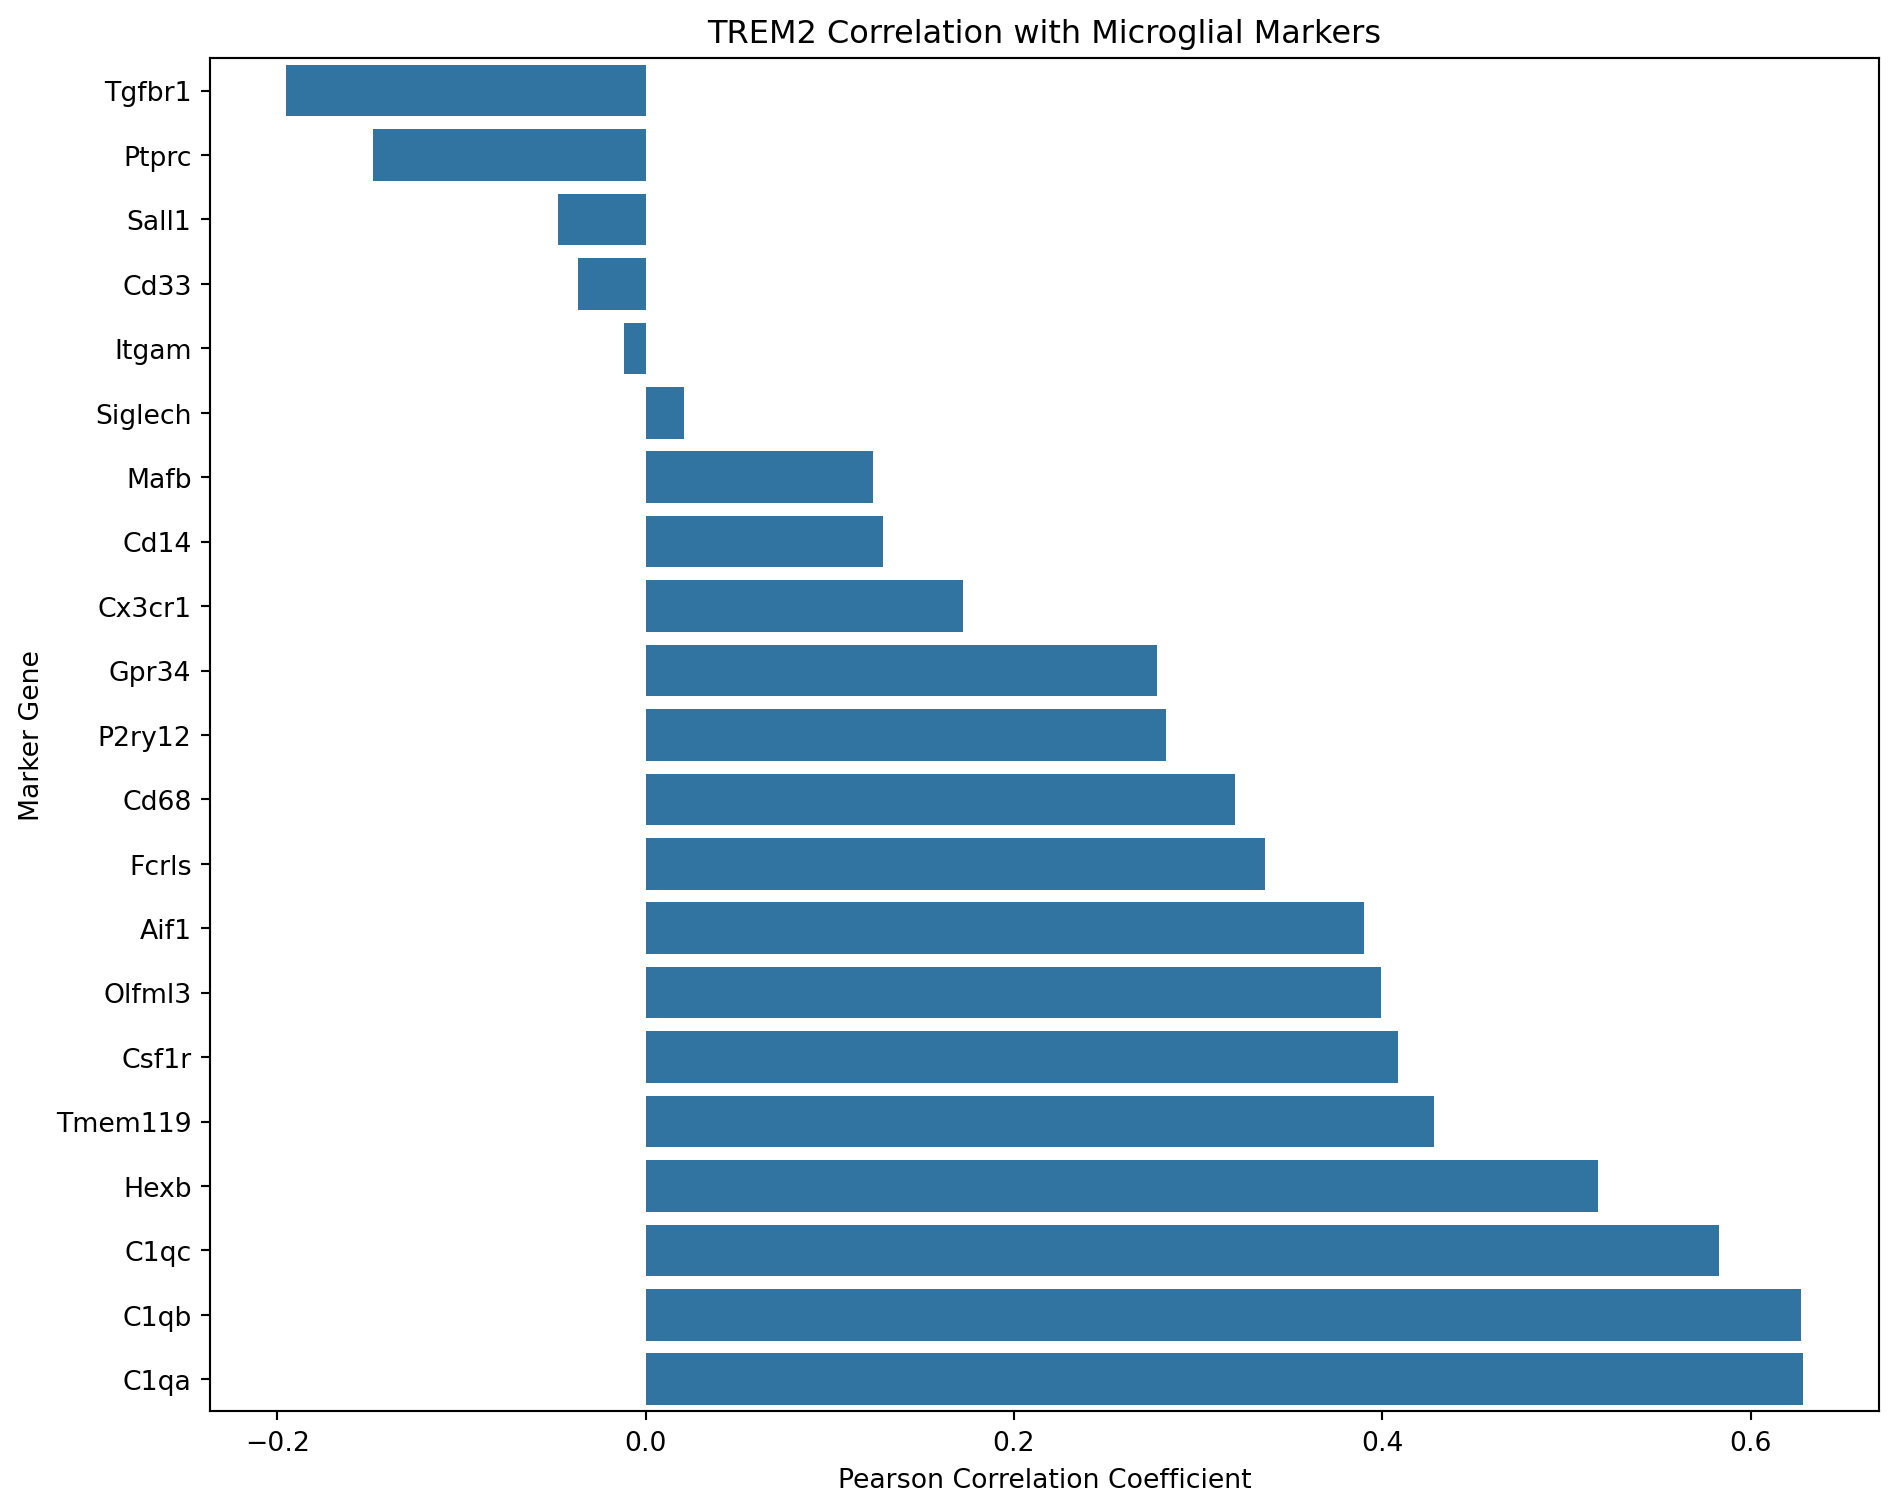
\includegraphics[keepaspectratio]{index_files/figure-latex/notebooks-eda-fig-trem2-correlations-output-1.png}}

}

\caption{\label{fig-trem2-correlations}Correlation analysis between
TREM2 and other microglial marker genes. Bar plot shows Pearson
correlation coefficients, ordered by strength of correlation. Positive
values indicate positive correlation, while negative values indicate
inverse relationships.}

\end{figure}%

\textsubscript{Source:
\href{https://EugOT.github.io/MicrogliaTRAP/notebooks/eda-preview.html\#cell-fig-trem2-correlations}{Comprehensive
analysis of hypothalamic microglia across multiple}}

\paragraph{Regional and Cluster-Specific
Patterns}\label{regional-and-cluster-specific-patterns}

The heatmap analysis (Figure~\ref{fig-trem2-cluster-enrichment-heatmap})
revealed distinct patterns of TREM2 expression across both regions and
clusters.

\begin{figure}[H]

\centering{

\pandocbounded{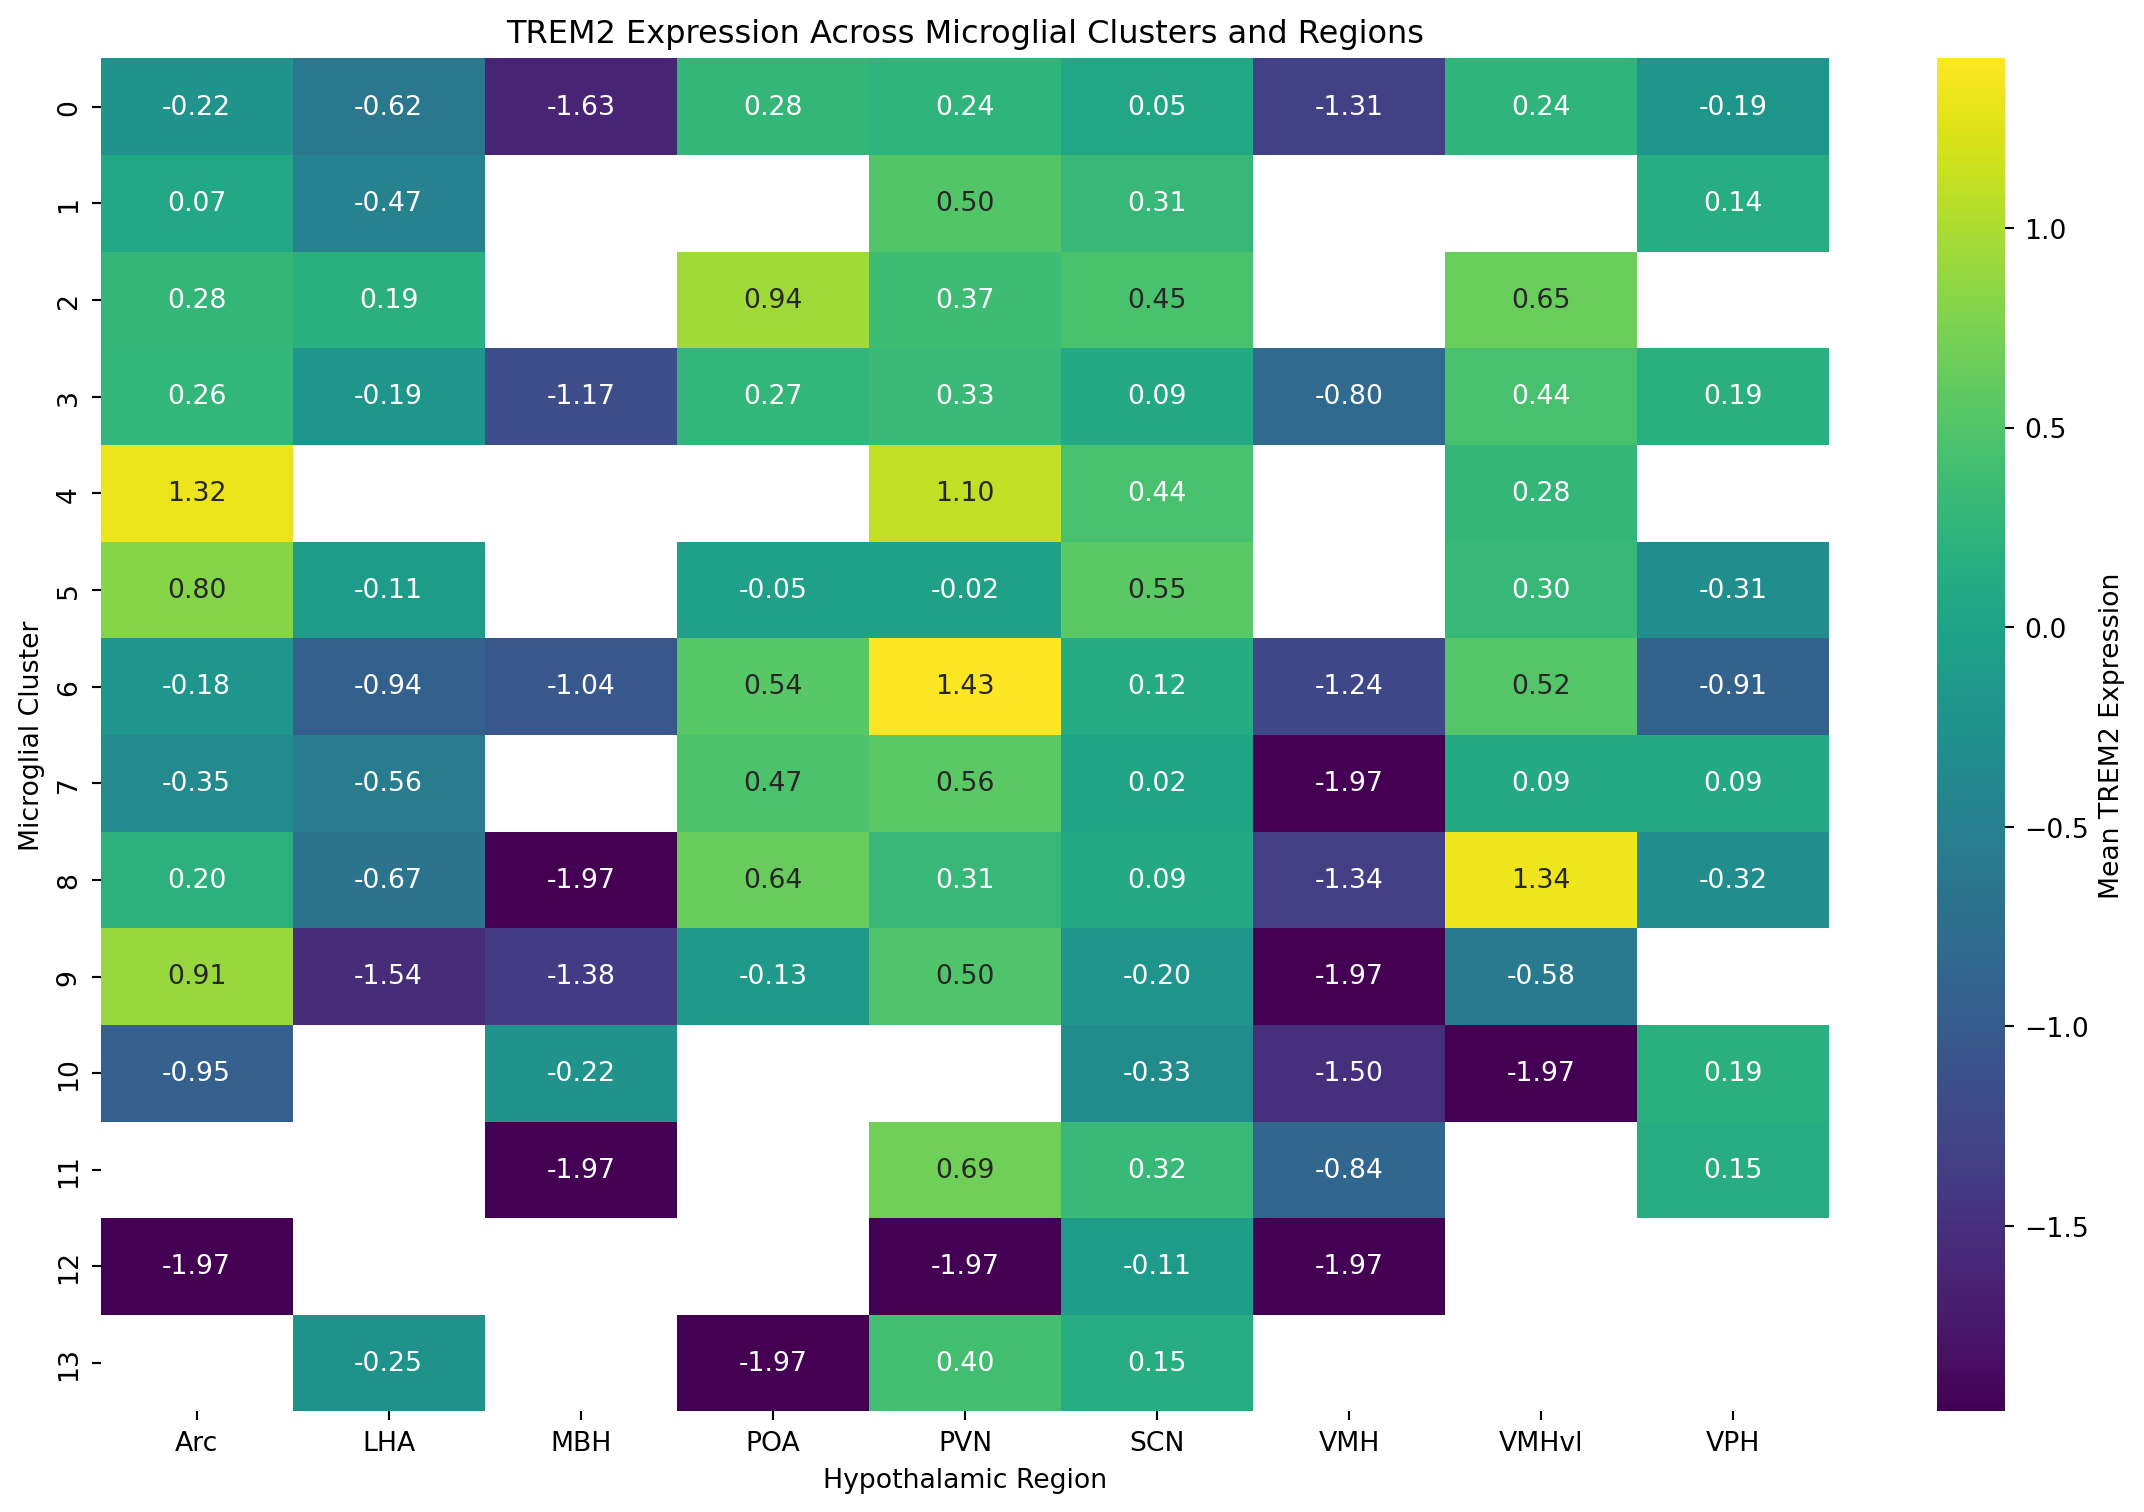
\includegraphics[keepaspectratio]{index_files/figure-latex/notebooks-eda-fig-trem2-cluster-enrichment-heatmap-output-2.png}}

}

\caption{\label{fig-trem2-cluster-enrichment-heatmap}Regional and
cluster-specific TREM2 expression patterns. Heatmap shows mean TREM2
expression levels across different microglial clusters (rows) and
hypothalamic regions (columns). Color intensity represents expression
level, with darker colors indicating higher expression.}

\end{figure}%

\textsubscript{Source:
\href{https://EugOT.github.io/MicrogliaTRAP/notebooks/eda-preview.html\#cell-fig-trem2-cluster-enrichment-heatmap}{Comprehensive
analysis of hypothalamic microglia across multiple}}

\paragraph{Molecular Interactions}\label{molecular-interactions}

The co-expression network analysis
(Figure~\ref{fig-trem2-coexpression-network}) identified key molecular
interactions of TREM2 with other genes.

\begin{figure}[H]

\centering{

\pandocbounded{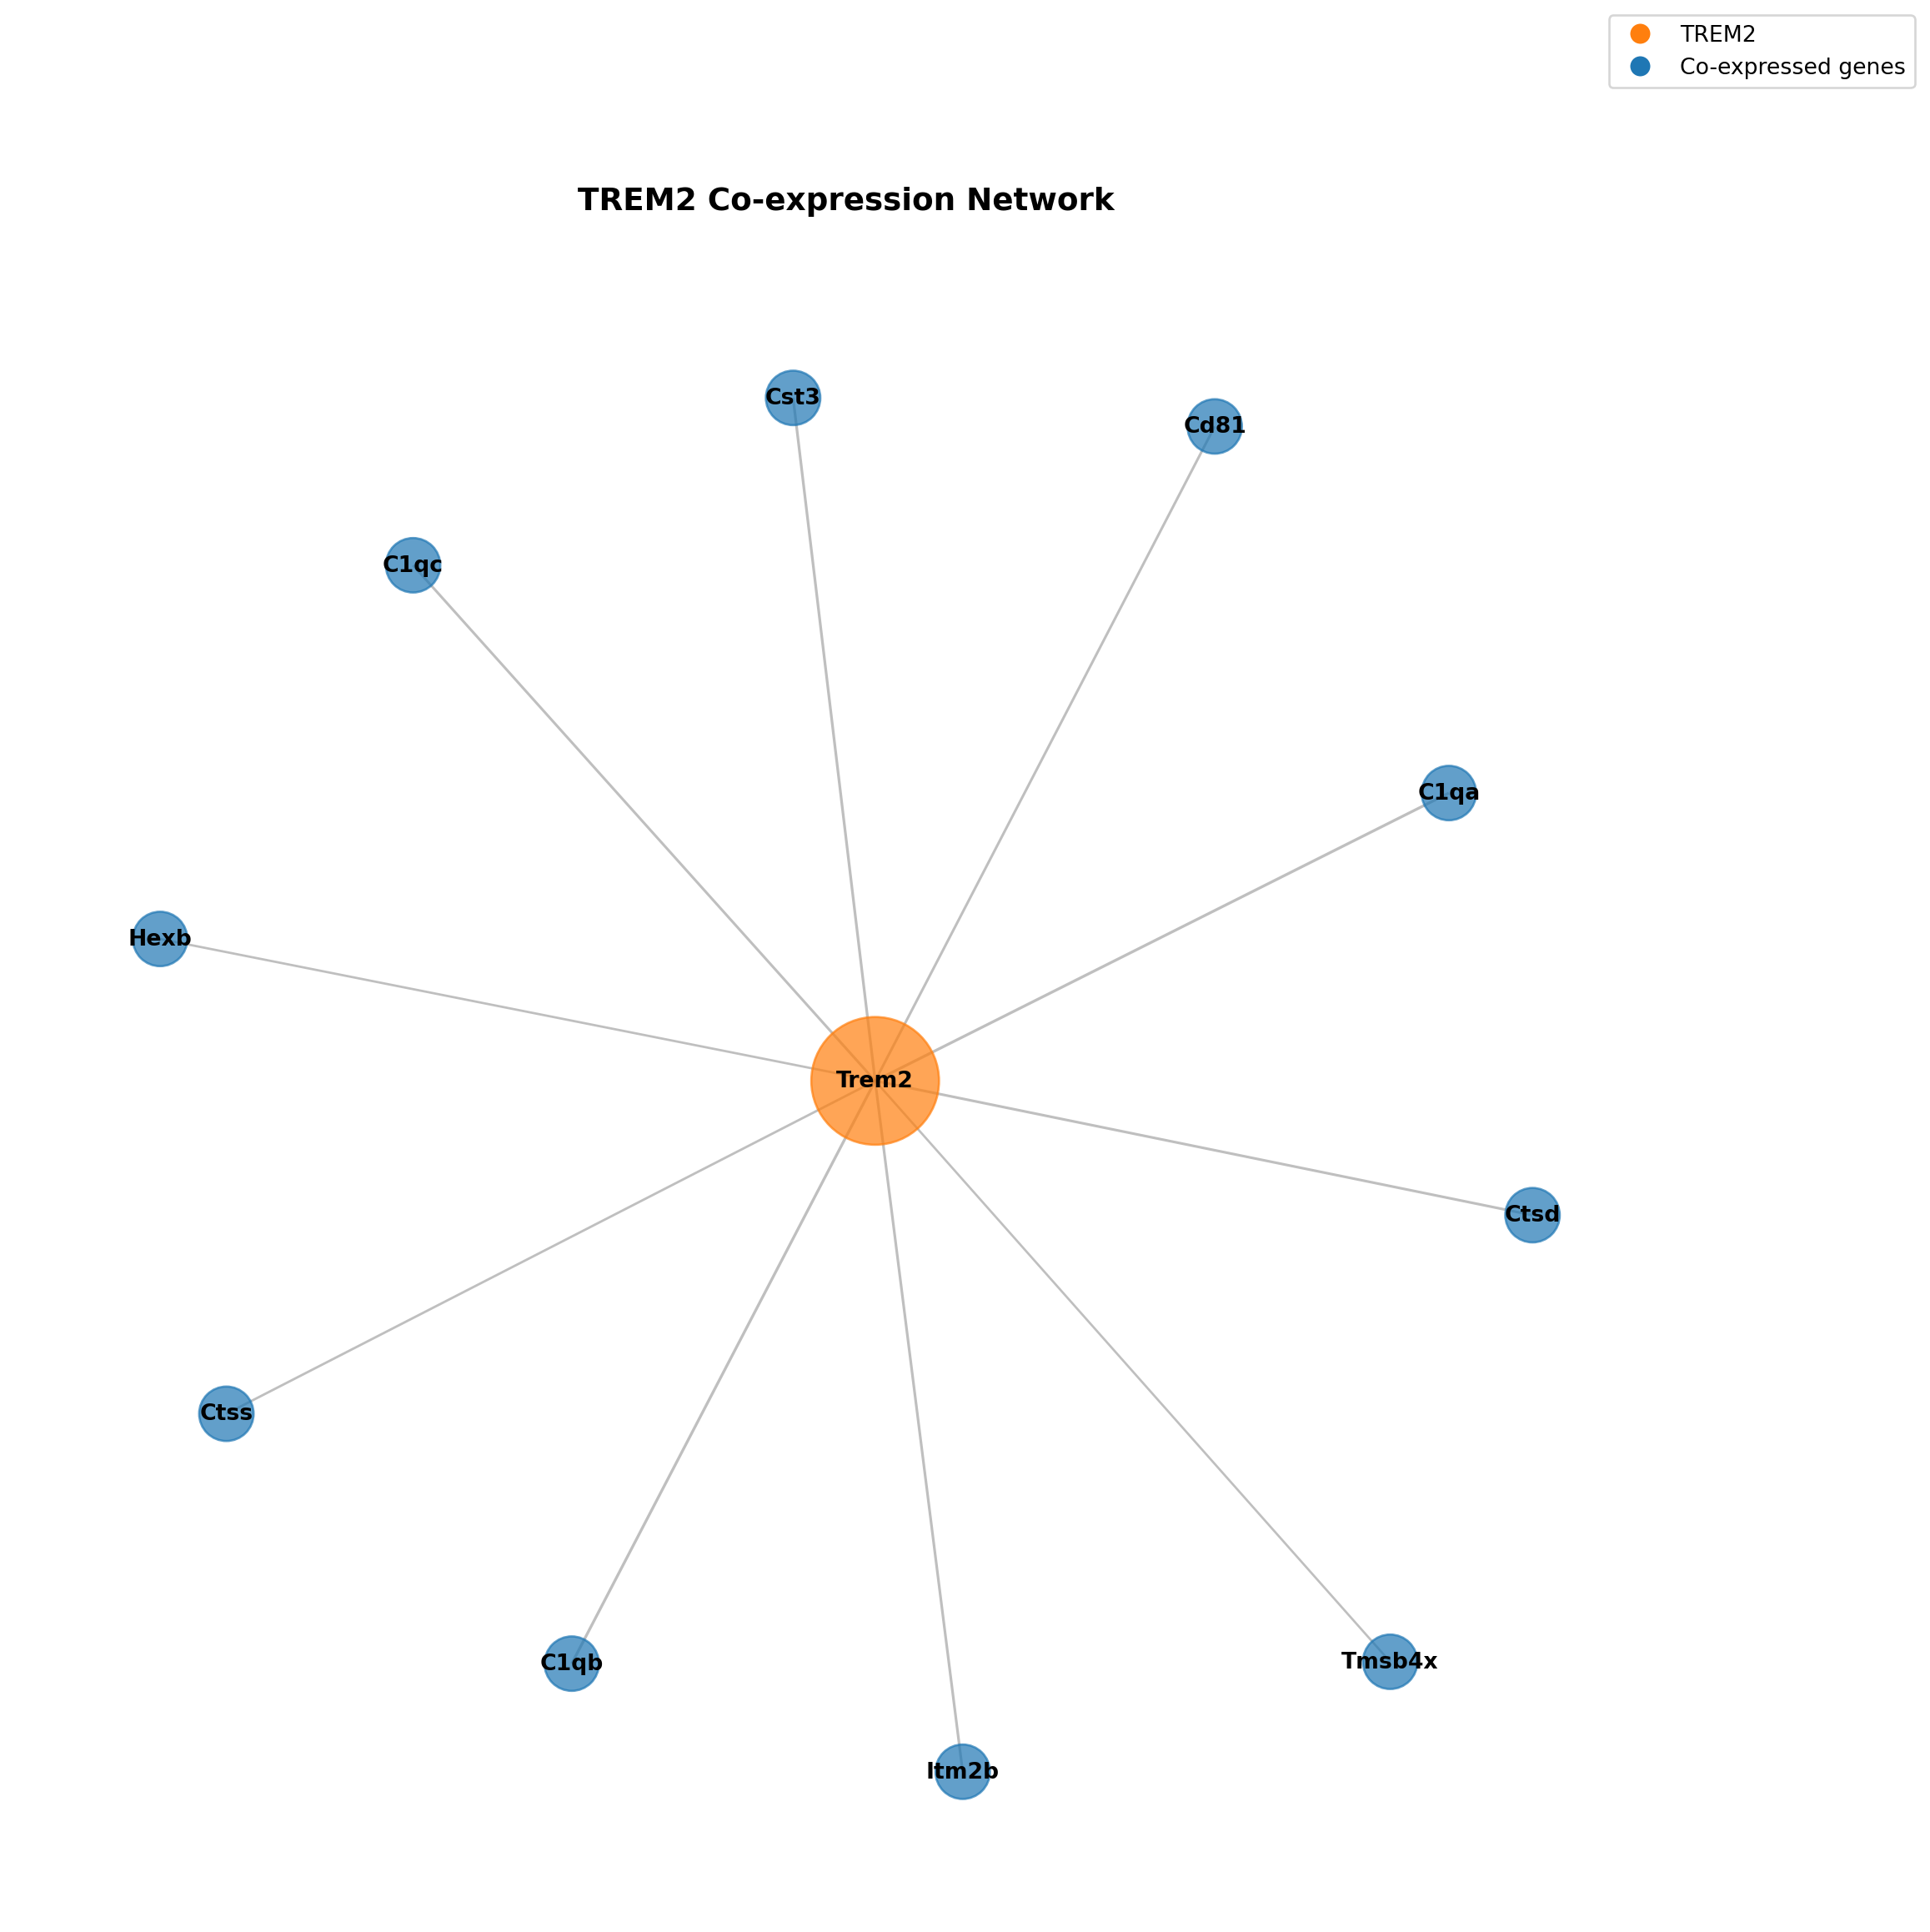
\includegraphics[keepaspectratio]{index_files/figure-latex/notebooks-eda-fig-trem2-coexpression-network-output-1.png}}

}

\caption{\label{fig-trem2-coexpression-network}TREM2 co-expression
network in hypothalamic microglia. Nodes represent genes, with TREM2 as
the central hub. Edge weights represent the absolute Pearson correlation
coefficient between gene pairs. Only correlations above 0.3 are shown.}

\end{figure}%

\begin{verbatim}

Network Statistics:
Number of co-expressed genes: 10
Number of connections: 10

Network Metrics:
Network density: 0.182
Average clustering coefficient: 0.000
\end{verbatim}

\textsubscript{Source:
\href{https://EugOT.github.io/MicrogliaTRAP/notebooks/eda-preview.html\#cell-fig-trem2-coexpression-network}{Comprehensive
analysis of hypothalamic microglia across multiple}}

\subsubsection{Statistical Analysis}\label{statistical-analysis}

Statistical comparison across regions
(Figure~\ref{fig-trem2-regional-stats}) revealed three distinct TREM2
expression domains:

\begin{figure}[H]

\centering{

\pandocbounded{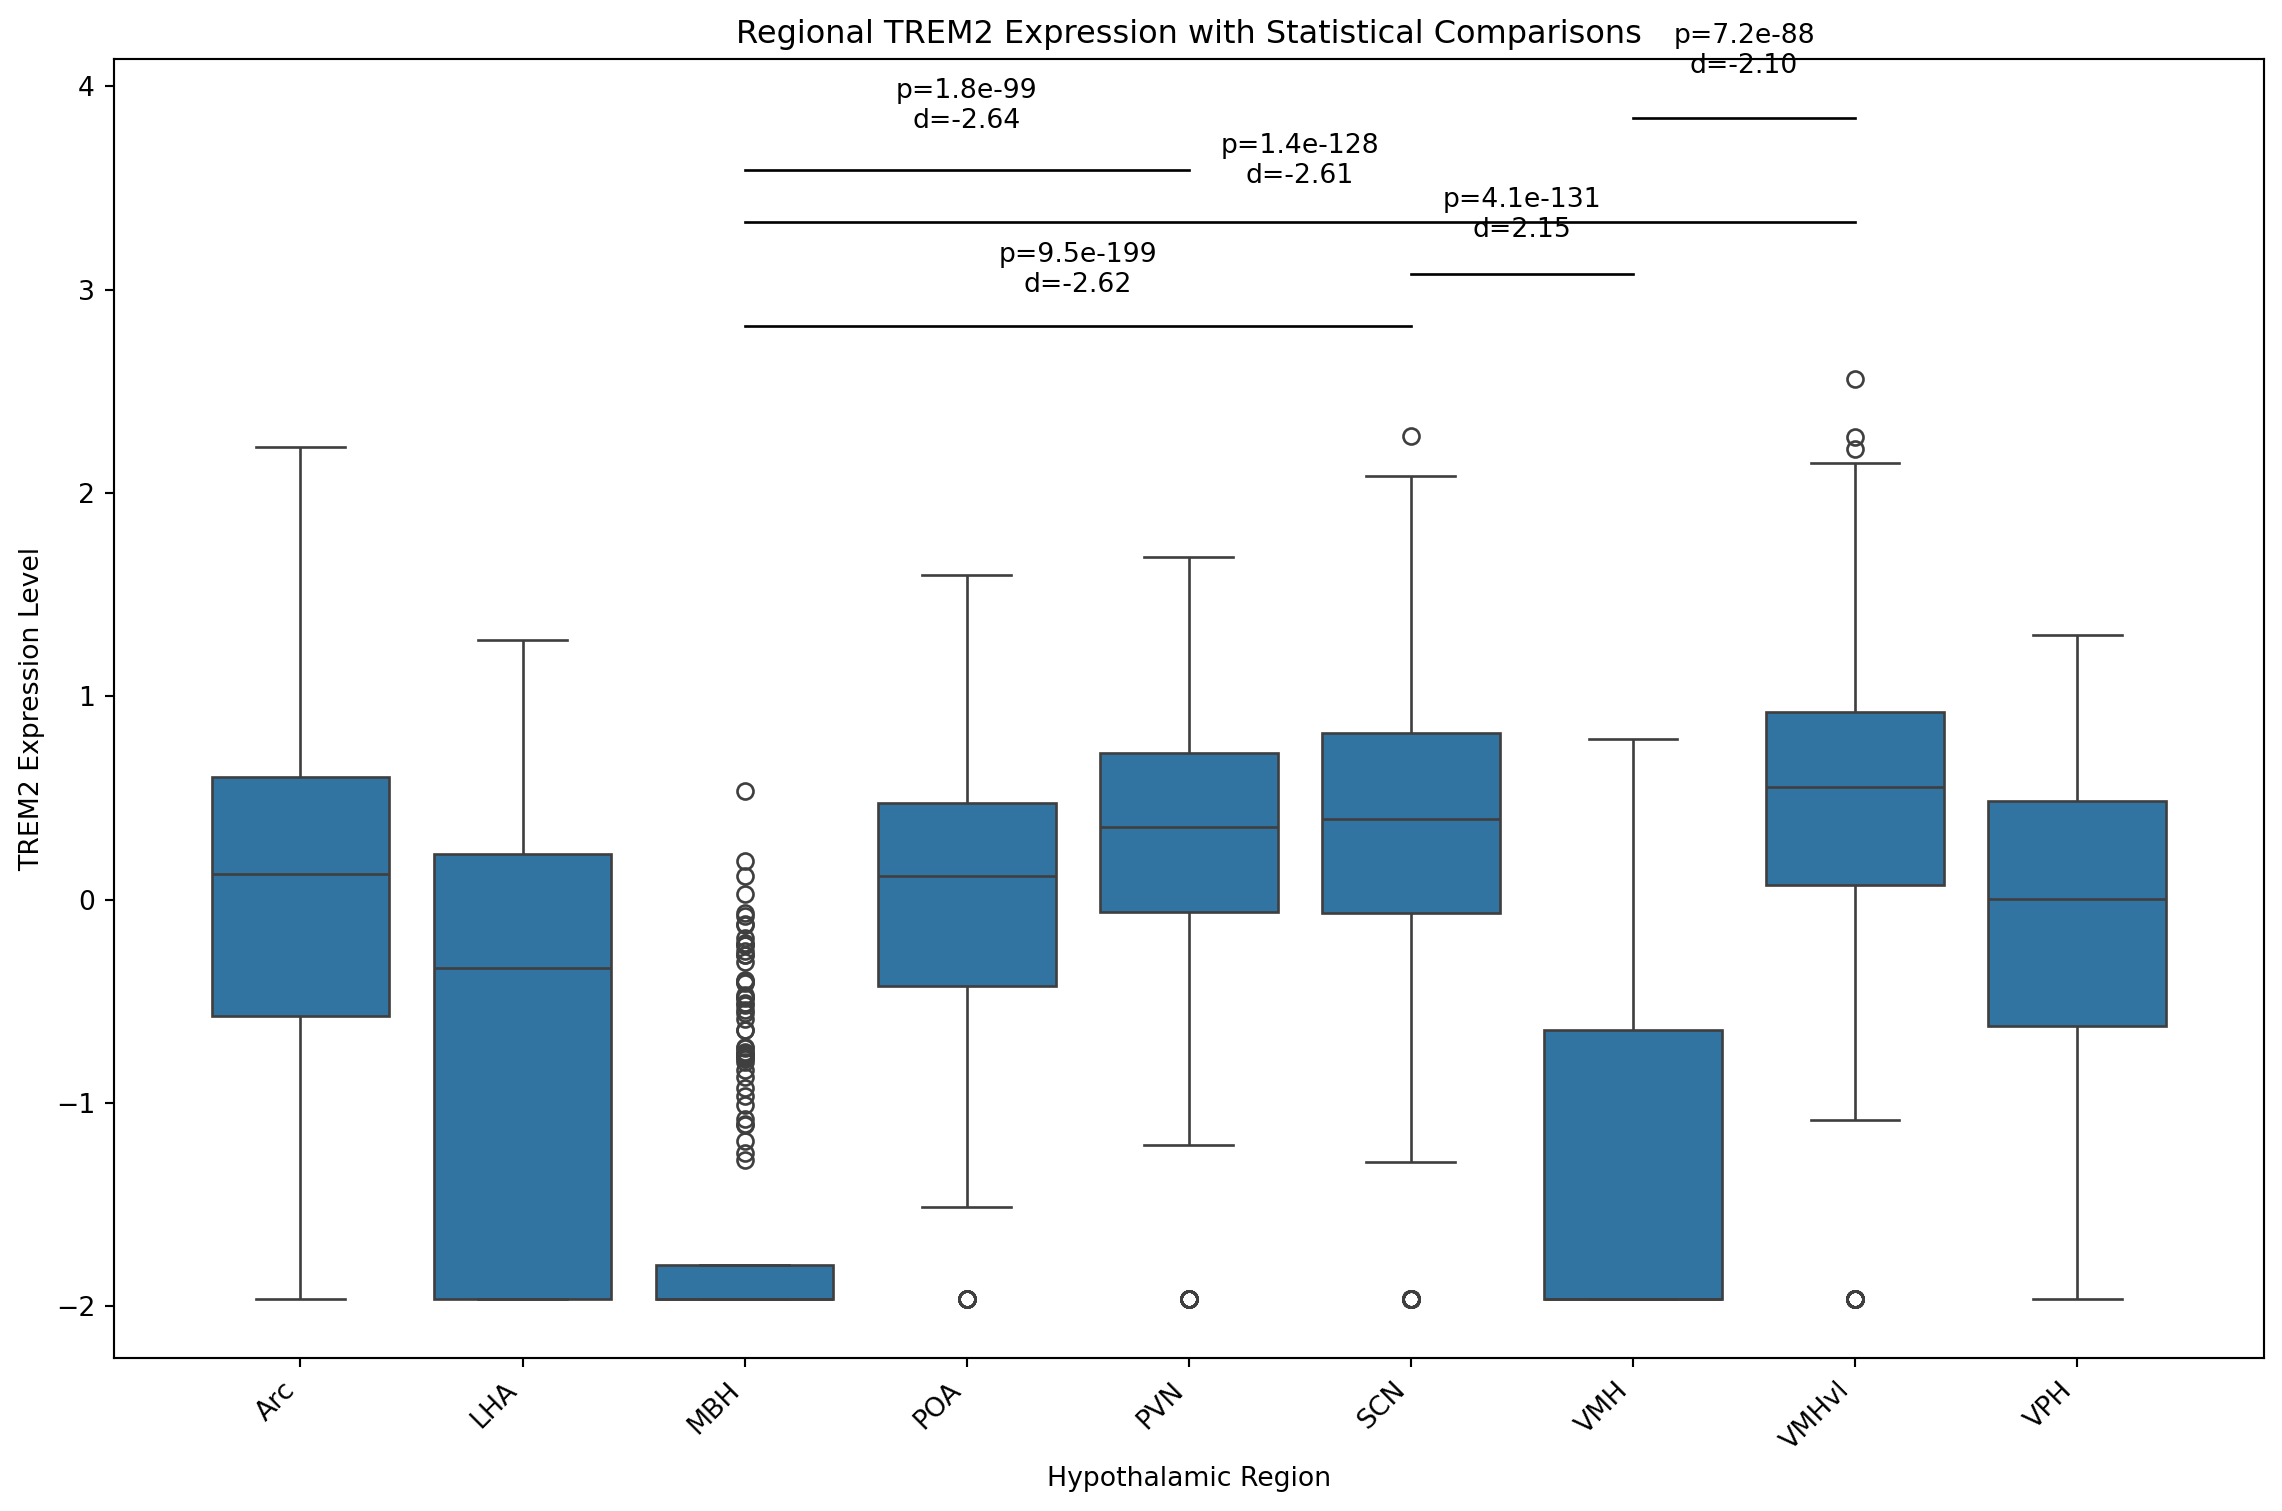
\includegraphics[keepaspectratio]{index_files/figure-latex/notebooks-eda-fig-trem2-regional-stats-output-1.png}}

}

\caption{\label{fig-trem2-regional-stats}Statistical comparison of TREM2
expression across hypothalamic regions. Box plots show the distribution
of TREM2 expression levels in each region. Significance bars indicate
the top 5 most significant pairwise comparisons (FDR-corrected
p-values). Cohen's d effect sizes are shown for each comparison,
quantifying the magnitude of expression differences between regions.}

\end{figure}%

\textsubscript{Source:
\href{https://EugOT.github.io/MicrogliaTRAP/notebooks/eda-preview.html\#cell-fig-trem2-regional-stats}{Comprehensive
analysis of hypothalamic microglia across multiple}}

\begin{enumerate}
\def\labelenumi{\arabic{enumi}.}
\tightlist
\item
  \textbf{High expression domain:} SCN, PVN, VMHvl (means \textgreater{}
  0.1)\\
\item
  \textbf{Intermediate expression domain:} POA, VPH, Arc (means between
  -0.3 and 0.1)\\
\item
  \textbf{Low expression domain:} MBH, MnPO, VMH (means \textless{}
  -0.9)
\end{enumerate}

The most significant differences were observed between:\\
- \textbf{MBH and SCN:} Cohen's d = -2.67, p-adj \textless{} 1e-300\\
- \textbf{SCN and VMH:} Cohen's d = 1.94, p-adj \textless{} 1e-300\\
- \textbf{MBH and PVN:} Cohen's d = -2.31, p-adj = 7.73e-158

\subsubsection{Interpretation}\label{interpretation}

The observed regional heterogeneity in TREM2 expression suggests
region-specific roles for microglial TREM2 signaling. The high
expression in the SCN and PVN---regions crucial for circadian rhythm and
neuroendocrine function---indicates potential involvement of TREM2 in
these processes. In contrast, the notably low expression in the MBH and
VMH (except ventro-lateral part) implies different functional states in
these subregions. Moreover, our super conservative filtering approach
(reducing 271,739 cells to 3,108 high-confidence microglia) and the
comprehensive use of well-defined gene lists ensure that only the most
robustly determined microglia are analyzed. The co-expression analysis
further implies potential molecular mechanisms by which TREM2 may
influence microglial function in distinct hypothalamic regions.

These findings provide a comprehensive map of TREM2 expression across
hypothalamic regions and suggest potential region-specific functions of
TREM2-expressing microglia in the hypothalamus.




\end{document}
